\section{Filtri}
\subsection{Filtri Ideali}
\lezione{Lezione 13}{11/11/2024}
I filtri ideali sono filtri descritti matematicamente e con proprietà difficilmente replicabili con esattezza
tramite circuiti reali.\\
Consideriamo un \textbf{Sistema senza Distorsione} nella seguente forma:
\begin{equation}
    y(t) = Ax(t - t_0)
\end{equation}
La trasformata di questo sistema è la seguente:
\begin{equation}
    Y(f) = AX(f)e^{-j2\pi ft_0} \tag{proprietà \eqref{prop: traslTempi}}
\end{equation}
Con $H(f) = Ae^{-j2\pi ft_0} = \begin{cases}
    |H(f)| = A\\
    \angle H(f) = (-2\pi t_0) f 
\end{cases}$
\subsection{Filtri Lineari Ideali}
Definiamo \textbf{Filtro Lineare Ideale} un filtro nella seguente forma:
\begin{equation}
    H(f) = \begin{cases}
        Ae^{-j2\pi ft_0} & \text{ se } f \in B\\
        0 & \text{ se } f \not\in B
    \end{cases}
\end{equation}
Dove $B$ è detta \textbf{Banda Passante di Un filtro}, perchè non annulla la frequenza del segnale in ingresso.

\subsubsection{Filtro Passa-Basso (Ideale)}
Questo filtro fa passare tutte le frequenze al di sotto di una \textbf{Frequenza di Taglio} $f_T$, ossia:
\begin{equation}
    H(f) = \begin{cases}
        Ae^{-j2\pi ft_0} & \text{ se } |f| < f_T\\
        0 & \text{ altrimenti}
    \end{cases}
\end{equation}
Possiamo calcolare la sua \textbf{risposta all'impulso} (Considerando $A = 1, t_0 = 0$):
\begin{equation*}
    H_{LP} = \begin{cases}
        1 & \text{ se } |f| < f_T\\
        0 & \text{ altrimenti}
    \end{cases} = \text{rect}\left(\frac{t}{2f_T}\right)
\end{equation*}
\begin{equation*}
    \underbrace{\text{rect}\left(\frac{f}{2f_T}\right)}_{H(f)} \fAnticouple \underbrace{2f_T\text{sinc}(2f_Tt)}_{h(t)}
\end{equation*}

\subsubsection{Filtro Passa-Alto (Ideale)}
Questo filtro fa passare, al contrario, tutte le frequenze al di sopra di una \textbf{Frequenza di Taglio} $f_T$, ossia:
\begin{equation}
    H(f) = \begin{cases}
        Ae^{-j2\pi ft_0} & \text{ se } |f| \geq f_T\\
        0 & \text{ altrimenti}
    \end{cases}
\end{equation}
Possiamo calcolare la sua \textbf{risposta all'impulso} (Considerando $A = 1, t_0 = 0$):
\begin{equation*}
    H_{HP} = \begin{cases}
        1 & \text{ se } |f| \geq f_T\\
        0 & \text{ altrimenti}
    \end{cases} = 1 - \text{rect}\left(\frac{t}{2f_T}\right)
\end{equation*}
\begin{equation*}
    \underbrace{1 - \text{rect}\left(\frac{f}{2f_T}\right)}_{H(f)} \fAnticouple \underbrace{\delta(t) - 2f_T\text{sinc}(2f_Tt)}_{h(t)}
\end{equation*}

\subsubsection{Filtro Passa-Banda (Ideale)}
Questo filtro fa passare tutte le frequenze entro un intervallo $\left[f_m,f_M\right]$, ossia:
\begin{equation}
    H(f) = \begin{cases}
        Ae^{-j2\pi ft_0} & \text{ se } f_m < |f| < f_M\\
        0 & \text{ altrimenti}
    \end{cases}
\end{equation}
Possiamo calcolare la sua \textbf{risposta all'impulso} (Considerando $A = 1, t_0 = 0$):
\begin{equation*}
    H_{BP} = \begin{cases}
        1 & \text{ se } f_m < |f| < f_M\\
        0 & \text{ altrimenti}
    \end{cases} = \text{rect}\left(\frac{f - f_c}{B}\right) + \text{rect}\left(\frac{f + f_c}{B}\right)
\end{equation*}
\begin{equation*}
    \underbrace{\text{rect}\left(\frac{f - f_c}{B}\right) + \text{rect}\left(\frac{f + f_c}{B}\right)}_{H(f)} \fAnticouple \underbrace{2B\text{sinc}(Bt)\cos(2\pi f_ct)}_{h(t)}
\end{equation*}

\subsubsection{Filtro Arresta-Banda (Ideale)}
Questo filtro fa passare, al contrario, tutte le frequenze al di fuori di un intervallo $\left[f_m,f_M\right]$, ossia:
\begin{equation}
    H(f) = \begin{cases}
        Ae^{-j2\pi ft_0} & \text{ se } \leq f_m \textbf{ o } |f| \geq f_M \\
        0 & \text{ altrimenti}
    \end{cases}
\end{equation}
Possiamo calcolare la sua \textbf{risposta all'impulso} (Considerando $A = 1, t_0 = 0$):
\begin{equation*}
    H_{BS} = \begin{cases}
        1 & \text{ se } f_m < |f| < f_M\\
        0 & \text{ altrimenti}
    \end{cases} = 1 - \text{rect}\left(\frac{f - f_c}{B}\right) - \text{rect}\left(\frac{f + f_c}{B}\right)
\end{equation*}
\begin{equation*}
    \underbrace{1 - \text{rect}\left(\frac{f - f_c}{B}\right) - \text{rect}\left(\frac{f + f_c}{B}\right)}_{H(f)} \fAnticouple \underbrace{\delta(t) - 2B\text{sinc}(Bt)\cos(2\pi f_ct)}_{h(t)}
\end{equation*}

\subsection{Filtri Reali}
I filtri reali, sono invece, quelli costruiti tramite componenti circuitali. I circuiti analogici, per chiare limitazioni fisiche,
non potranno mai riprodurre fedelmente i comportamenti dei filtri ideali.
\subsubsection{Circuito RC}
Il circuito RC corrisponde ad un \textbf{Filtro Passa-Basso Reale} per il fatto che la risposta all'impulso assomiglia
a quella di un filtro passa-basso. In un circuito possiamo immaginare un impulso come una scarica di intensità infinita
che attraversa il circuito in un tempo infinitesimo e carica il condensatore instantaneamente di $1A$, e poi si scarica seguendo
un andamento \textbf{esponenziale decrescente} (circa). La risposta all'impulso possiamo descriverla cosi:
\begin{equation}
    h(t) = u(t)e^{-\frac{t}{RC}}
\end{equation}
Con $R$ la \textbf{resistenza del circuito} e $C$ la \textbf{capacità del condensatore}. $RC$ viene detto \textbf{tempo caratteristico} del sistema.
La trasformata di questa risposta all'impulso è la seguente:
\begin{equation*}
    H(f) = \frac{1}{1 + j2\pi f RC}
\end{equation*}
Se consideriamo la frequenza di taglio $f_T = \frac{1}{2\pi RC}$ abbiamo che:
\begin{equation}
    H(f) = \frac{1}{1 + j\frac{f}{f_T}}
\end{equation} 
Analizziamo modulo e frequenza di questa risposta in frequenza:
\begin{equation}
    |H(f)| = 
    \begin{cases}
        1 &\text{ se } f \ll f_T\\
        \frac{1}{\sqrt{2}} &\text{ se } f = f_T \\
        \ll 1 &\text{ se } f \gg f_T   
    \end{cases}
\end{equation}
\begin{equation}
    \angle H(f)= 
    \begin{cases}
        \approx 0 &\text{ se } f \ll f_T\\
        -\frac{\pi}{4} &\text{ se } f = f_T \\
        -\frac{\pi}{2} &\text{ se } f \gg f_T   
    \end{cases}
\end{equation}
Il grafico di risposta all'impulso dovrebbe essere:
\begin{center}
    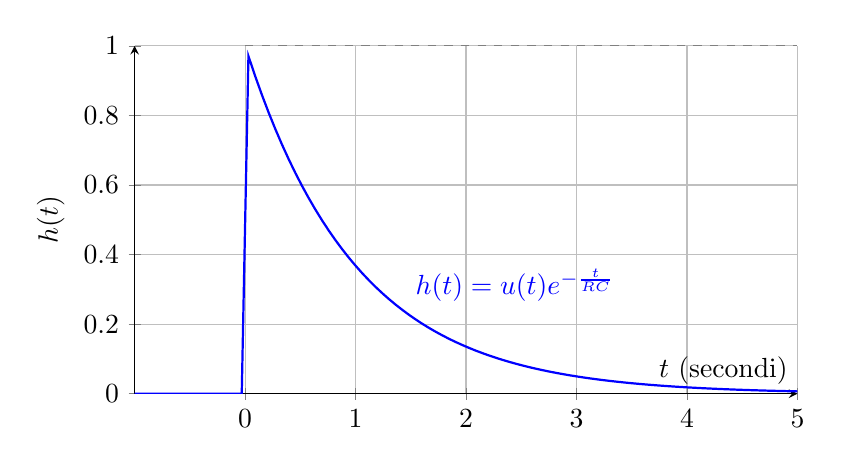
\begin{tikzpicture}
        \begin{axis}[
            width=10cm, height=6cm,
            xlabel={$t$ (secondi)},
            ylabel={$h(t)$},
            xmin=-1, xmax=5,
            ymin=0, ymax=1,
            xtick={-1,0,1,2,3,4,5},
            ytick={0,0.2,0.4,0.6,0.8,1},
            grid=both,
            domain=-1:5,
            samples=100,
            axis x line=middle, % Sposta l'asse x al centro
            axis y line=left, % Lascia l'asse y a sinistra
            legend pos=north east
        ]
        
        % Grafico della scarica del condensatore con condizione a zero per t<0
        \addplot[blue, thick] {x < 0 ? 0 : exp(-x)} node[pos=0.5, above right] {$h(t) = u(t)e^{-\frac{t}{RC}}$};
        
        % Linea per V0
        \addplot[dashed, gray] coordinates {(0,1) (5,1)};
        \node at (axis cs:0.2,1) [anchor=south west] {$V_0$};
    
        \end{axis}
    \end{tikzpicture}
\end{center}
Dal momento che per $f > f_T$ la risposta in frequenza decresce per $1/f$ ogni volta, questo filtro viene detto
\textbf{filtro del I ordine}. 
\paragraph{Ordine n-esimo di un Filtro.}Si definisce Ordine n-esimo di un Filtro, un filtro che decresce al di fuori
della banda di $1/f^n$ 